%----------------------
% metodicky pokyn
%----------------------
\newpage
\pagestyle{plain}
%\setfonts [CMRoman/10]
\thispagestyle{plain}
\input{podminkyPrihlasovani.tex}
\newpage
\SekceFmt{��seln� k�dov�n� vzd�l�vac�ch program�}
\textbf{Orientace v~��seln�m k�dov�n� vzd�l�vac�ch program�}\\

Identifika�n� k�d vzd�l�vac� akce je �estim�stn� a m� n�sleduj�c� strukturu:\hspace{5mm} \fbox{A--BB--C--DD}\\[5mm]
%\begin{center}
V�znam jednotliv�ch ��sel k�du:\\[3mm]
\begin{tabular}{|c|l|}
\hline
pozice & v�znam\\ \hline
*A & k�d pracovi�t� 1--5\\
BB & oborov� skupina 0--15\\
C & pololet� p��slu�n�ho �koln�ho roku 1--2\\
DD & po�adov� ��slo v~r�mci pracovi�t� a oborov� skupiny\\
\hline
\end{tabular}\\
\begin{tabbing}
*A -- k�d pracovi�t�:\hspace{2mm}\= 1 -- Hradec Kr�lov�\\
\> 2 -- Trutnov\\
\> 3 -- Rychnov nad Kn�nou\\
\> 4 -- Ji��n\\
\> 5 -- N�chod\\
\end{tabbing}
P��klad:\hspace{5mm} \fbox{2--03--1--15}\\[3mm]
\begin{tabular}{|c|l|}
\hline
pozice & v�znam\\ \hline
2 & pracovi�t� Trutnov\\
03 & oborov� skupina �j a literatura\\
1 & 1. pololet� �koln�ho roku\\
15 & 15. akce v~oborov� skupin� �j a literatura\\
\hline
\end{tabular}\\
%\end{center}

\vfill
%\begin{frameenv}
%\begin{center}
\fcolorbox{tmava}{svetla}
{\parbox[b]{.9\textwidth}{\centering \Large\bf P�ihlaste se na vzd�l�vac� program:\\ \Ustav\\[3mm]{\Huge\bf \Web}}}
%\end{center}
%\end{frameenv}

%\vfill 
%\begin{center} 
%\textbf{Um�st�n� PgC v~Hradci Kr�lov�}\\[4mm]
% mapka - PgC
%\fbox{
%\scalebox{.8}{%
%\includegraphics{pgc_mapa}
%}}
%\end{center}

%-------------------------
% metodicky pokyn - Bara
%-------------------------
%\newpage
%\pagestyle{plain}
%%\setfonts [CMRoman/10]
%\thispagestyle{plain}
%\newcommand{\obrazovka}[3]{%
\begin{figure}[#3]
\begin{center}
\fbox{\includegraphics[scale=.4]{#1}}
\caption{#2}
\end{center}
\end{figure}
%\par
}
\SekceFmt{Pr�vodce elektronickou p�ihl�kou}\par
\par\noindent
Pro vyhled�n� informac� o~vzd�l�vac� akci pou�ijte vyhled�vac� obrazovku. Po�adovanou akci je mo�n� vyhledat p��mo podle jej�ho identifika�n�ho k�du. 

Identifika�n� k�d vzd�l�vac� akce je �estim�stn� a m� n�sleduj�c� strukturu: \fbox{A--BB--C--DD}\\
\begin{center}
V�znam jednotliv�ch ��sel k�du:\\
\begin{tabular}{|c|l|}
\hline
pozice & v�znam\\ \hline
A~& k�d pracovi�t�\\
BB & oborov� skupina\\
C & pololet� �koln�ho roku\\
DD & po�adov� ��slo v~r�mci pracovi�t� a oborov� skupiny\\
\hline
\end{tabular}\\
\end{center}
Pokud chcete vyhledat akci p��mo podle jej�ho k�du, zad�te ��slo do vyhled�vac�ho boxu bez poml�ek.

Nezn�te-li ��slo akce a chcete zobrazit akce ur�it�ho pracovi�t�, pou�ijte odkazy v~sekci \uv{�len�n� akc� podle pracovi�t�}. Pokud chcete zobrazit akce ur�it� oborov� skupiny, pou�ijte odkazy v~sekci \uv{�len�n� vzd�l�vac�ch akc� po oborech}.
\obrazovka{scr1x}{Vyhled�n� vzd�l�vac� akce}{h}
\newpage
M�te-li po�adovanou akci zobrazenou v~seznamu vyhledan�ch akc�, tak pro zobrazen� detailn�ch informac� o~akci klikn�te na n�zev akce.
\obrazovka{scr2x}{Zobrazen� vyhledan�ch akc�}{h}\par
Na obrazovce zobrazuj�c� podrobnosti o~vzd�l�vac� akci je ve spodn� ��sti um�st�na tabulka s~term�ny akce. Pokud jsou na akci je�t� p�ij�m�ny p�ihl�ky, je mo�n� prov�st elektronick� p�ihl�en� na vybran� term�n. Jedn�--li se o~cyklickou akci, p�ihl�ka se prov�d� pouze na prvn� term�n cyklu, na ostatn� term�ny jste p�ihl�eni automaticky. 

V~��dku tabulky term�nu se nach�z� je�t� ikonka pro zobrazen� pozv�nky a p�ihl�ky ve form�tu HTML (form�t ur�en� pro tisk na tisk�rn�) a ikonka pro vygenerov�n� pozv�nky a p�ihl�ky ve form�tu PDF. Tento form�t doporu�ujeme z~d�vod� lep�� typografick� kvality a snadn�j��ho tisku. Pro pr�ci s~form�tem PDF pot�ebujete alespo� zdarma ���en� prohl��e� \textit{Acrobat Reader} od firmy Adobe.
\obrazovka{scr3x}{Podrobnosti vzd�l�vac� akce}{h}
\newpage
Pro zd�rn� vypln�n� elektronick� p�ihl�ky je kl��ov� spr�vn� vyplnit �vodn� box, kde je po�adov�no rodn� ��slo a IZO �kolsk�ho za��zen�. Rodn� ��slo je citliv� osobn� �daj, nicm�n� pro bezprobl�mov� vyhled�n� Va�� bezhotovostn� platby je d�le�it�. Na�e organizace m� regitraci na �OO� a m��e tedy s~t�mto �dajem pro svoji vnit�n� pot�ebu disponovat. Zad�n� rodn�ho ��sla nen� kontrolov�no, je tedy mo�n�, v~p��pad� va�� neochoty tento �daj poskytnout, zadat libovoln� �et�zec (��seln� nebo znakov�). Budete--li ov�em akci hradit bezhotovostn�, je nezbytn� tento v� identifik�tor sd�lit na�emu ekonomick�mu odd�len� pro dohled�n� va�� platby a dan� ��slo si zapsat a pou��vat p�i p�ihla�ov�n� i na dal�� akce.

Druh�m �dajem je IZO �koly. Pokud nezn�te IZO va�� �koly, m��ete se pokusit jej vyhledat v~na�� \textit{datab�zi �kol}, p��padn� tam IZO va�� �koly doplnit. Pokud nejste na akci vysl�n ��dn�m �kolsk�m za��zen�m, zadejte znak *.

Pokud zad�te IZO pouze ��ste�n�, budete na dal�� obrazovce vyzv�ni vybrat �kolu z~na�� datab�ze p�esn�.
\obrazovka{scr4x}{Za��tek elektronick� p�ihl�ky}{h}
P�ihl�ka pokra�uje vypln�n�m dal��ch pot�ebn�ch �daj�. Pokud jste se ji� v~minulosti ��astnil(a) n�jak� na�� akce a sv��il(a) n�m sv� rodn� ��slo, budete  ji� m�t v�t�inu �daj� p�edvypln�n�ch. Je mo�n� �daje opravit a doplnit. Je nutn� vyplnit alespo� povinn� �daje, kter� jsou zobrazeny �ervenou barvou.
\obrazovka{scr5x}{Vypln�n� po�adovan�ch �daj� p�ihl�ky}{h}
\newpage
Posledn� obrazovka zobrazuje potvrzen� va�� �sp�n� p�ihl�ky. V�nujte pozornost zvl�t� �daj�m pro bezhotovostn� platbu.
\obrazovka{scr6x}{Potvrzen� p�ihl�ky}{h}\par
Cel� informa�n� syst�m pedagogick�ho centra, s~jeho� ve�ejn� p��stupnou ��st� jsme v�s pr�v� sezn�mili, vyu��v� v�hradn� OSS (Open Source Software) - tedy sofware ���en� pod licenc� GNU/GPL, jinak �e�eno zdarma. 

Informa�n� syst�m je naprogramov�n jazyky PHP a Perl, tiskov� v�stupy jsou generov�ny typografick�m syst�mem \LaTeX (repektive pdf\LaTeX) do form�tu PDF. Jako datov� �lo�i�t� je vyu��v�n datab�zov� server MySQL. Sazba tohoto zpravodaje je vytv��ena typografick�m syst�mem \LaTeX a v�sledn�m form�tem pro tisk je PostScript. 

V��e zmi�ovan� software vyu��v� prost�ed� opera�n�ho syst�mu Linux. Pokud byste m�li z�jem dozv�d�t se v�ce o~jeho vyu�it� na va�� �kole, jste zv�ni na semin��:
\vfill
\begin{minipage}{\textwidth}
\begin{ovalenv}\setfonts [Lido-crm/10]
\Large
{\centering
\parpic[c][ct]%
{\scalebox{.7}{
\includegraphics{images/edunix}}} 
\picskip{0}\par}
\vspace{5mm}
{\centering
T�m Edunixu, IC Gymn�zium Bo�eny N�mcov�, PgC Hradec Kr�lov�\\
ve spolupr�ci s~ostatn�mi organizacemi\\
p�ipravuj�\\[3mm]
\textbf{\Huge Konference Linux a OSS/FS\\[2mm] ve �kolstv�}\\[3mm]
Konference na t�ma vyu�it� Linuxu, svobodn�ho software (FS) a otev�en�ho software (OSS) ve �koln�ch s�t�ch a u�ebn�ch. 
M�sto a term�n konference bude up�esn�n, p�edb�n� je stanovena na ��jen--listopad 2004.
Up�esn�n� term�nu a dal�� informace nalezneta na serverech:\\
\texttt{http://www.edunix.cz}\\
\texttt{http://www.gybon.cz/edunix}\\[2mm]}
\end{ovalenv}
\end{minipage}


%--------------------------------
% oraganizacni struktura - pavouk
%--------------------------------
%\newpage	
%\SekceFmt{Organiza�n� struktura}
\vspace{2cm}
\begin{center}
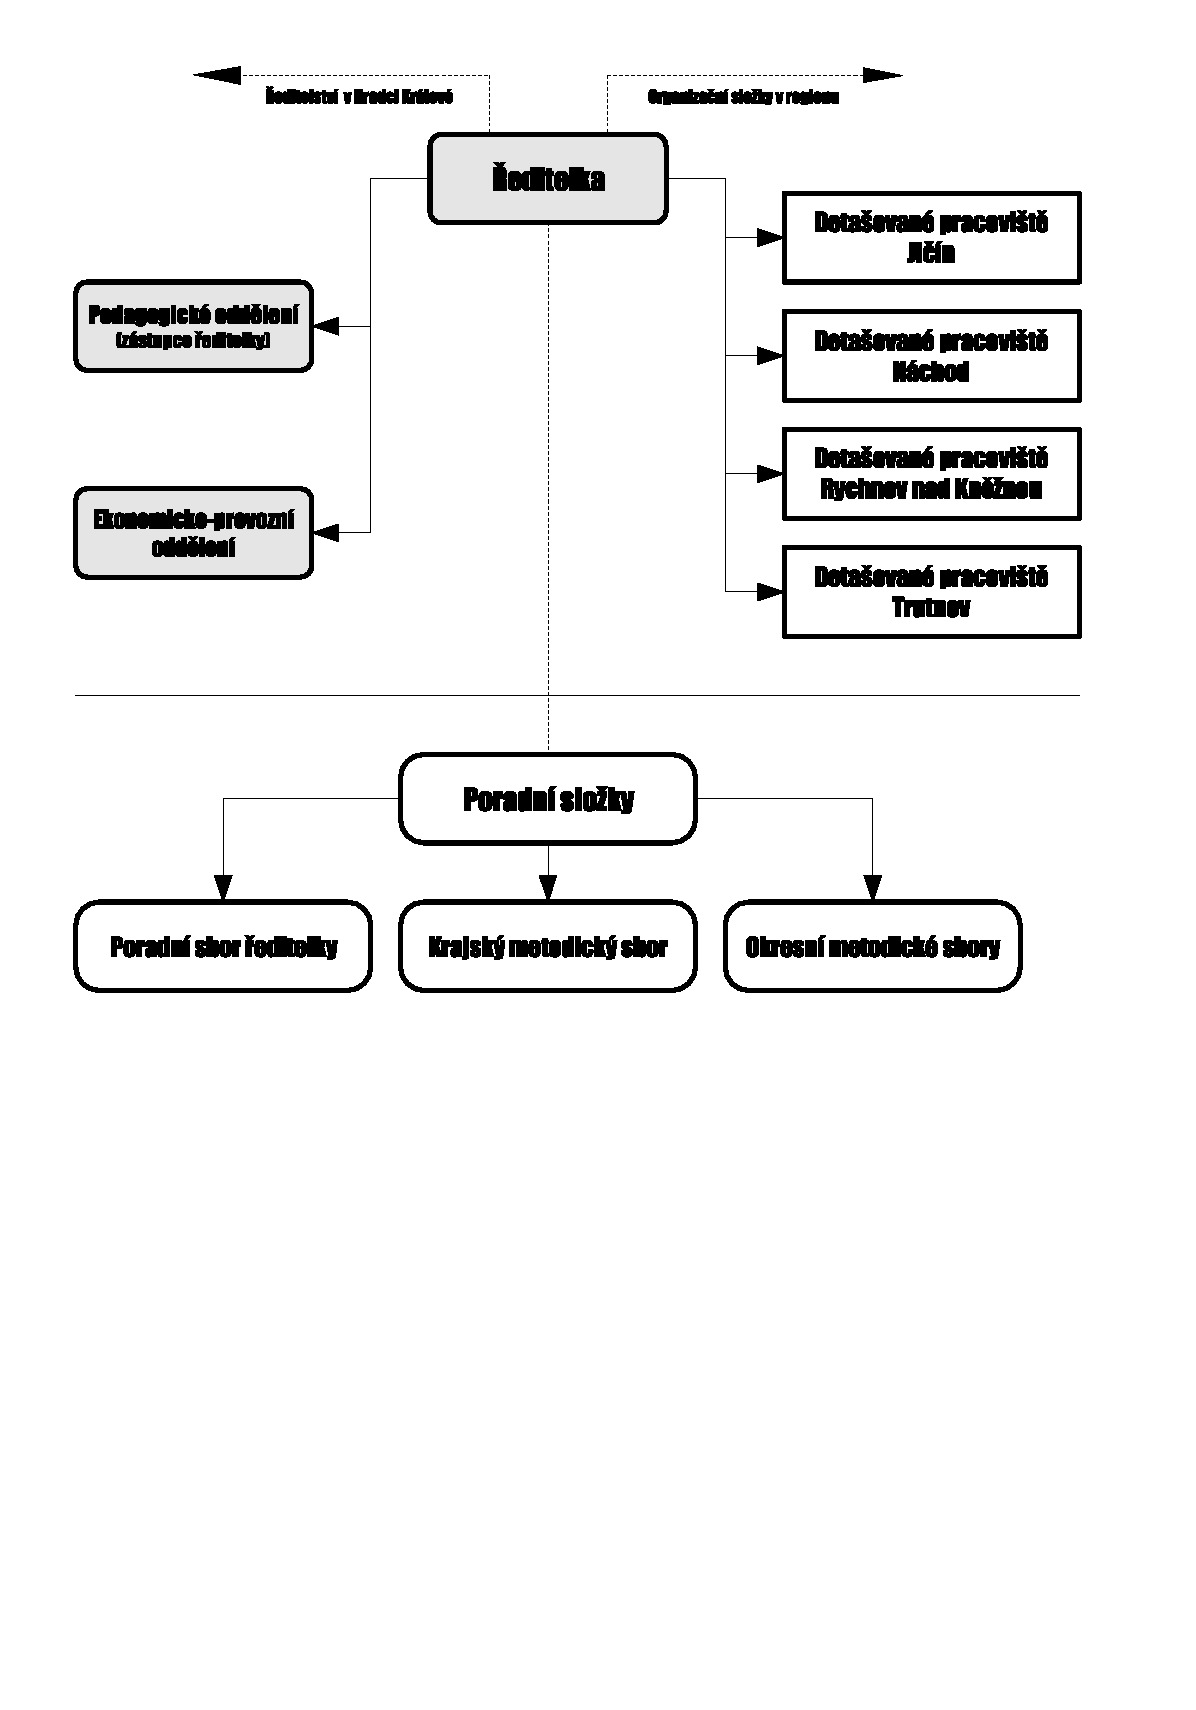
\includegraphics[scale=.89]{images/struct}
\end{center}

%----------
% interni pracovnici
%----------
\newpage
%\setfonts [CMRoman/10]
%\SekceFmt{P�ehled intern�ch pracovn�k�}
\newlength{\prvniTab}
\newlength{\druhyTab}
\setlength{\prvniTab}{7cm}
\setlength{\druhyTab}{8cm}
%
\vspace{3cm}
\textbf{�editelka/�editel:}\\
\begin{tabbing}
\hspace{\prvniTab}\=\hspace{\druhyTab}\=\kill
Dle v�sledku konkurzn�ho ��zen�\\
%Mgr. Bc. Marcela Nov�kov�\>metodi�ka DVPP\>prac. HK\\
\end{tabbing}
%\textbf{Z�stupkyn� �editelky:}\\
%\begin{tabbing}
%\hspace{\prvniTab}\=\hspace{\druhyTab}\=\kill
%Bc. Eva Kuncov�\>metodi�ka DVPP, vedouc� pracovi�t�,\>prac. JC\\
%\>vedouc� pedagogick�ho odd�len�\>\\
%\end{tabbing}
\textbf{Pedagogick� odd�len�:}\\
\begin{tabbing}
\hspace{\prvniTab}\=\hspace{\druhyTab}\=\kill
%Mgr. Dagmar Kone�n�\>metodi�ka DVPP\>prac. HK\\
%Ing. Zuzana Pustinov�\>metodi�ka DVPP, spr�vkyn� pracovi�t�\>prac. TU\\
Mgr. Mark�ta Mr�zkov�\>metodi�ka DVPP, vedouc� pracovi�t�\>prac. NA\\
%Mgr. Alena Ro�kov�\>metdodi�ka DVPP,\>prac. TU\\
%\>referentka sout�� a p�ehl�dek\>\\
Ing. Stanislava Stierandov�\>metodi�ka DVPP, vedouc� pracovi�t�\>prac. TU\\
%Mgr. Hana ��pkov� \>metodi�ka DVPP\>prac. RK\\
%Mgr. Veronika �t�p�nov�\>metodi�ka DVPP, spr�vkyn� pracovi�t�\>prac. NA\\
%Mgr. Eva �reibrov�\>metodi�ka DVPP, vedouc� pracovi�t�\>prac. RK\\
%Mgr. Eva Vol�kov�\>metodi�ka DVPP\>prac. HK\\
Bc. et Bc. Marcela Pavlov�\>metodi�ka DVPP\>prac. HK\\
%Mgr. Ji�� Zeman\>metodik DVPP, spr�vce pracovi�t�\>prac. RK\\
%Mgr. Zorka �elezn�\>metodi�ka DVPP\>prac. HK\\
\end{tabbing}
\textbf{Ekonomicko-provozn� odd�len�:}\\
\begin{tabbing}
\hspace{\prvniTab}\=\hspace{\druhyTab}\=\kill
So�a Brz�kov�\>sekretari�t �editelstv�, vedouc� pracovi�t�,\>prac. HK\\
\>vedouc� odd�len�\>\\
Vladislav He�man\>��etn�\>prac. HK\\
%Alena Stanislavov�\>administrativn� pracovnice\>prac. NA\\
Jana Svat�\>personalistka, mzdov� ��etn�\>prac. HK\\
%Mark�ta �olcov�\>��etn�\>prac. HK\\
\end{tabbing}
\textbf{Odd�len� sout�� a p�ehl�dek:}\\
\begin{tabbing}
\hspace{\prvniTab}\=\hspace{\druhyTab}\=\kill
Mgr. Dana Ber�kov�\>koordin�torka sout�� a p�ehl�dek,\>prac. HK\\
\>vedouc� odd�len�\>\\
%Bc. Tereza Lomnick�\>referentka sout�� a p�ehl�dek,\>prac. RK\\
%\>vedouc� pracovi�t�\>\\
%Bc. Jana N�vltov�\>referentka sout�� a p�ehl�dek\>prac. NA\\
%\>vedouc� pracovi�t�\>\\
%Mgr. Alena Zme�kalov� (Ro�kov�)\>referentka sout�� a p�ehl�dek\>prac. TU\\
%\>metodi�ka DVPP\>\\
Drahoslava �enat�\>referentka sout�� a p�ehl�dek\>prac. JC\\
\end{tabbing}
\textbf{Projekt I-KAP:}\\
\begin{tabbing}
\hspace{\prvniTab}\=\hspace{\druhyTab}\=\kill
Luk� Nov�k\>metodik aktivit\>prac. HK\\
\end{tabbing}



%----------
% kontakty
%----------
\newpage
%\setfonts [CMRoman/10]
\SekceFmt{Jak se spojit:\\ \Ustav}
%
\begin{tabbing}     
\hspace{6cm}\= \kill
\bf I�O:\>62731882\\
\bf Bankovn� spojen�:\>Komer�n� banka Hradec Kr�lov�\\
\tab\>��et �. 8195410267/0100\\
\bf Internet:\>\url{\Web/}\\
\end{tabbing}
% 
% ---------------- Hradec --------------------
%
\nadpisprac{\Ustav\\pracovi�t� Hradec Kr�lov�}
\begin{tabbing}     
\hspace{6cm}\= \kill
\bf S�dlo pracovi�t�:\>Na Okrouhl�ku 1371/30, 500 02 Hradec Kr�lov�\\
%\tab\>(v are�lu Z� �tef�nikova -- zadn� pavilon vpravo)\\
\bf Telefonn� ��slo:\>495 514 804 -- tel. / fax, mobil: 722 569 521\\
%\tab\>495 514 636\\
%\tab\>495 514 805\\
%\tab\>495 514 806 -- fax\\
%\tab\>495 500 918 -- koordin�tor ICT\\
\bf E-mail:\>\url{hradec@kkivi.cz}\\
\end{tabbing}
%Pracovi�t� Hradec Kr�lov� se nach�z� ve 2. pat�e prav�ho zadn�ho pavilonu Z� �tef�nikova ul. na Moravsk�m p�edm�st�. Od termin�lu HD z n�stupi�t� D2 linkou MHD �. 24, vystoupit na zast�vce HV�ZDA (11. zast�vka od termin�lu, 10. od vlak. n�dra��), nebo �. 9, vystoupit na t�e zast�vce (10. zast�vka od termin�lu, 9. od vlak. n�dra��), proj�t are�lem prodejny sm�rem k Z�, p�ed schody k hlavn�mu vchodu do Z� zabo�it doprava, pokra�ovat st�le pod�l plotu sm�rem k Sp� pro sluchov� posti�en�, u domku ve �koln� zahrad� zabo�it vraty doleva a pokra�ovat po chodn�ku ke vchodu do pavilonu po prav� stran�. Od vchodu do pavilonu rovn� ke schod�m, vyj�t do 2. patra a d�t se doprava. Od are�lu HV�ZDA je cesty zna�ena 2 sm�rovkami.\\
\nadpistab{Kontakty na pracovn�ky -- pracovi�t� Hradec Kr�lov�}
\tblb
Ing. Jaroslav Jir�sko & \url{reditel@kkivi.cz} & 724 913 220 \\
Mgr. Dana Ber�kov� & \url{berakova@kkivi.cz} & 495 514 804, 725 059 837 & dana.berakova\\
%So�a Brz�kov� & \url{brzakova@kkivi.cz} & 495 514 804, 722 569 521 & sona.brzakova\\
Martin Hepnar & \url{hepnar@kkivi.cz} & 495 514 804, 722 569 521 \\
Vladislav He�man & \url{herman@kkivi.cz} & 495 514 804, 733 645 784 & vladislav.herman \\
%Hana �i�m�rov� (ext.)& \url{cizmarova@kkivi.cz} & 495 514 804 & 732 481 765 \\
%Mgr. Dagmar Kone�n� & \url{konecna@kkivi.cz} & 495 514 804 & \url{d.konecna} \\
%Mgr. Jaroslav Nov�k (ext.) & \url{novak@kkivi.cz} & 732 409 282 & \tab \\
Bc. Jana Kav��kov� & \url{kavrikova@kkivi.cz} & 724 775 911 \\
Ing. Mgr. Milu� Mat�jcov� & \url{matejcova@kkivi.cz} & 603 717 049 \\
Luk� Nov�k & \url{novak@kkivi.cz} & 722 971 995 \\
%Mgr. Bc. Marcela Nov�kov� & \url{novakova@kkivi.cz} & 495 514 805, 777 340 408 & marcela.novakova3\\
Bc. et Bc. Marcela Pavlov� & \url{pavlova@kkivi.cz} & 722 569 512 \\
%Jana Svat� & \url{svata@kkivi.cz} & 495 514 804, 722 457 124 & j.svata \\
%Mark�ta �olcov� & solcova@kkivi.cz} & 495 514 804 & \tab \\
%Mgr. Jana Pol��kov� (ext.)& \url{polackova@kkivi.cz} & 495 500 913 & 777 210 899\\
%Ing. Ond�ej Rusek (ext.) & \url{rusek@gybon.cz} & \tab & \tab\\
%Mgr. Lenka Tak��ov� (ext.)& \url{takacova@kkivi.cz} & 721 635 756 & \tab \\
%Eva Tom�t�kov� & tomastikova@kkivi.cz & 495 500 915 & \tab \\
%Mgr. Eva Trenzov� (ext.)& \url{trenzova.e@seznam.cz} & 736 454 956 & \tab \\
%Mgr. Milu�e Urbanov� & urbanova@kkivi.cz & 495 500 910, 495 514 636 & 605 268 135\\
%Luk� Vod�k & vodak@kkivi.cz & 495 514 804 & \tab \\ 
Mgr. Jakub Sofka & \url{sofka@kkivi.cz} & 722 569 514 \\
Bc. Lucie Val�kov� & \url{valaskova@kkivi.cz} \\
Mgr. Eva Vol�kov� (ext.)& \url{volakova@kkivi.cz} & 495 514 804, 777 340 409 & eva.volakova2 \\
Luk� Tepl�& \url{teply@kkivi.cz} & 607 046 856 \\
%Hana Zyklov� & zyklova@kkivi.cz & \tab & 777 019 411\\
%Mgr. Hana �ate�kov� & zateckova@kkivi.cz & 495 500 913, 495 514 804 & 604 289 434\\
%Mgr. Zorka �elezn�& zelezna@kkivi.cz & 495 514 804 & 605 811 075\\
\tble
% 
% ------------- Jicin ------------
%
\nadpisprac{\Ustav\\pracovi�t� Ji��n}
\begin{tabbing}     
\hspace{6cm}\= \kill
\bf S�dlo pracovi�t�:\>Komensk�ho n�m. 45, 506 01 Ji��n\\
\bf Telefonn� ��slo:\>724 882 650\\
\bf E-mail:\>\url{zenata@kkivi.cz}\\
\end{tabbing}
%Pracovi�t� Ji��n se nach�z� v~p��zem� Z� �eleznick� ul. u~nemocnice. Z~autobusov�ho n�dra�� sm�rem k~Ji��nsk� br�n�, p�ed br�nou odbo�it doprava, rovn� Tylovou ulic�, p�es p�echod u~VZP do �eleznick� ulice.\\
%Pracovi�t� Ji��n se nach�z� v~p��zem� 4. Z� v~�eleznick� ulici �. 460 pobl�� nemocnice. Z~autobusov�ho n�dra�� sm�rem k~Ji��nsk� br�n�, p�ed br�nou odbo�it doprava, rovn� Tylovou ulic� a p�es p�echod u~VZP do �eleznick� ulice.\\
Pracovi�t� Ji��n se nach�z� v 1. pat�e VO� a SP� Ji��n, Komensk�ho  n�m. 45. Z autobusov�ho n�dra�� sm�rem na Vald�tejnovo n�m�st�, pokra�ovat ulic� Palack�ho sm�rem dol�, odbo�it vlevo na Komensk�ho n�m�st�.
\nadpistab{Kontakty na pracovn�ky -- pracovi�t� Ji��n}
\tblb
%PaedDr. Vladim�r Kauck� (ext.) & \url{kaucky@kkivi.cz} & 724 882 650 & \tab \\
%Mgr. Iva L�ftnerov� (ext.) & \url{luftnerova@kkivi.cz} & 724 882 650 & \url{luftniv}\\
%Bc. Eva Kuncov� & \url{kuncova@kkivi.cz} & 722 569 514 & \url{eva.kuncova3}\\
%Alena Matohl�nov�	&  \url{matohlinova@kkivi.cz} & 493 549 129 & 737 758 570\\
Drahoslava �enat� & \url{zenata@kkivi.cz} & 724 882 650 & \url{DRAZA194}\\
\tble\par
%
\newpage
\noindent
%
% -------------- Nachod --------------
%
\nadpisprac{\Ustav\\pracovi�t� N�chod}
\begin{tabbing}     
\hspace{6cm}\= \kill
\bf S�dlo pracovi�t�:\>Smi�ick�ch 1237, 547 01 N�chod\\
\bf Telefonn� ��slo:\>724 882 652\\
\bf E-mail:\>\url{nachod@kkivi.cz}\\
\end{tabbing}
Pracovi�t� N�chod se nach�z� v are�lu pedagogicko-psychologick� poradny (p��zem�  samostatn� vchod vpravo). Od autobusov�ho n�dra�� sm�r s�dli�t� Plhov, u samoobsluhy zabo�it doleva a pokra�ovat sm�r z�mek ulic� Smi�ick�ch. P�i pot�eb� zaparkov�n� auta zabo�te v kopci (sm�r z�mek) doprava do s�dli�t�, pokra�ujte kolem M� Plhov a hned za n� odbo�te doleva k parkovi�t� u PPP.\\
\nadpistab{Kontakty na pracovn�ky -- pracovi�t� N�chod}
\tblb
%PhDr. Jaroslava N�vltov� (ext.) & \url{nyvltova@kkivi.cz} & 491 419 159 & 491 428 744\\
%Mgr. Zden�k Pol�k (ext.) & \url{polak@kkivi.cz} & 491 419 159 & 491 423 243\\
%Mgr. Eva Cupalov� & \url{cupalova@kkivi.cz} & 491 422 437 & \tab \\
%Mgr. Lenka Proke�ov� (ext.) & \url{prokesova@kkivi.cz} &  491 422 437 & \tab\\
%Leo� Pol�ek (ext.) & \url{polasek@kkivi.cz} & 491 422 437, 491 422 416 & \tab \\
%Miroslava Jirkov� & \url{jirkova@kkivi.cz} & 491 422 437, 491 422 416 & \tab \\
%Alena Stanislavov� & \url{stanislavova@kkivi.cz} & 491 422 416 & \tab \\
%Mgr.\,Mark�ta Mr�zkov� & \url{mrazkova@kkivi.cz} & 722 569 515 & \url{mrazkovama} \\
%Mgr.\,Mark�ta\,Mr�zkov� & \url{mrazkova@kkivi.cz} & 722 569 515 & \url{mrazkovama} \\
%Bc.\,Jana N�vltov� (ext.) & \url{nyvltova@kkivi.cz} & 724 882 652 & \tab \\ %  \url{cheeky.girl}\\
%Mgr. Veronika �t�p�nov� & \url{stepanova@kkivi.cz} & 491 428 345, 722 569 515 & \url{veronika\_stepanova}\\
Bc. Kate�ina Krti�kov�, DiS. & \url{krtickova@kkivi.cz} & 722 569 515 & \tab \\
\tble
%
% ----------------- Rychnov ---------------
%
%\nadpisprac{Kontakty na  pracovn�ky -- Rychnov nad Kn�nou}
%\begin{tabbing}     
%\hspace{6cm}\= \kill
%\bf S�dlo pracovi�t�:\>Javornick� 1501, 516 01 Rychnov nad Kn�nou\\
%\bf Telefonn� ��slo:\>724 882 643\\
%\bf E-mail:\>\url{rychnov@kkivi.cz}\\
%\end{tabbing}
%Pracovi�t� Rychnov nad Kn�nou se nach�z� v~ulici Javornick� 1501, 2. vchod, p��zem�, sm�rem od st�edu m�sta mezi SOU Javornick� ul. (budova na k�i�ovatce) a Z� Rychnov n. Kn., Javornick� 1596.\\
%Pracovi�t� Rychnov nad Kn�nou se nach�z� v~p��zem� budovy v~Javornick� ulici �. 1501 (2. vchod), kter� je um�st�na mezi budovami VO� a SP�  pracovi�t� Javornick� ulice �. 1228 (b�val� SOU) a Z� v~Javornick� ulici �. 1596.\\
\nadpistab{Kontakty na pracovn�ky -- Rychnov nad Kn�nou}
\tblb
%Bc. Daniela Hartmanov� (ext.) & \url{hartmanova@kkivi.cz} & 494 534 377 & \tab\\
%Milu�e Moln�rov� & \url{molnarova@kkivi.cz} & 494 534 377 & \tab\\
%Bc. Tereza Lomnick� (ext.) & \url{lomnicka@kkivi.cz} & 724 882 643 & \tab\\
%gr. Hana ��pkov� & \url{sipkova@kkivi.cz} & 722 457 124 & \url{ha.sipkova} \\
%\tab & \tab & 724 882 643 & \tab\\
Bc. et Bc.  Marcela Pavlov� & \url{pavlova@kkivi.cz} & 722 569 512 & \tab \\
Bc. Petra Vo�lajerov� & \url{soutezerychnov@kkivi.cz} & 724 882 643 & \tab \\
%Mgr. Ji�� Zeman (ext.)& \url{zeman@kkivi.cz} &  737 307 827 & \url{jiri.zeman3}\\
\tble
%
% -------------------- Trutnov --------------------
%
\nadpisprac{\Ustav\\pracovi�t� Trutnov}
\begin{tabbing}     
\hspace{6cm}\= \kill
\bf S�dlo pracovi�t�:\>L�pov� 223, 541 01 Trutnov\\
\bf Telefonn� ��slo:\>720 516 096\\
\bf E-mail:\> \url{trutnov@kkivi.cz}\\
\end{tabbing}
%Pracovi�t� Trutnov se nach�z� v~budov� Obchodn� akademie Trutnov na Mal�m n�m�st� u~mostu p�es �eku.
%Z~vlakov�ho n�dra�� se d�t vlevo po chodn�ku u~hlavn� silnice. Po cca 200 m p�ej�t silnici k~�ece a p�es most p��mo p�ed budovu Obchodn� akademie. Od autobusov�ho n�dra�� k~�ece, pod�l vody ve sm�ru toku doj�t po promen�d� k~Obchodn� akademii (cca 500 m).\\
%Pracovi�t� Trutnov se nach�z� v~budov� obchodn� akademie na Mal�m n�m�st� �. 158 u~mostu p�es �eku. Z~�elezni�n�ho n�dra�� se d�t vlevo po chodn�ku pod�l hlavn� silnice, po cca 200 m p�ej�t silnici k~�ece a p�es most p��mo p�ed budovu obchodn� akademie. Od autobusov�ho n�dra�� pokra�ovat sm�rem k~�ece, d�le pod�l toku �eky doj�t cca 500 m po promen�d� k~obchodn� akademii.\\
Pracovi�t� Trutnov se nach�z� v budov� Poradensk�ho a vzd�l�vac�ho centra Trutnov. Z vlakov�ho n�dra�� pokra�ovat vlevo po chodn�ku u hlavn� silnice. Po cca 200 m p�ej�t silnici a most, doj�t ke Svatojansk�mu n�m�st�. D�le Barv��skou ulic� a p�ed parkovi�t�m K���ov� n�m. odbo�it vlevo a proj�t na konec ulice L�pov�. Od autobusov�ho n�dra�� doj�t po promen�d� kolem obchodn�ho domu M�j k parkovi�ti K���ov� n�m. Odbo�it vlevo a proj�t na konec ulice L�pov�.
\nadpistab{Kontakty na pracovn�ky -- pracovi�t� Trutnov}
\tblb
%Mgr. Petr Jind�ich & \url{jindrich@kkivi.cz} & 499 840 054 & 737 306 759\\
%Mgr. Jana Pol��kov� & \url{polackova@kkivi.cz} & 499 840 054 & 737 306 759\\
%Ing. Zuzana Pustinov� & \url{pustinova@kkivi.cz} & 499 840 054 & 720 516 096\\
%Jitka Barton��kov� (ext.)& \url{bartonickova@kkivi.cz} & 725 059 786 & \tab \\
Ing. Stanislava Stierandov� & \url{stierandova@kkivi.cz} & 720 516 096 & \url{stierandova}\\
Mgr. Alena Zme�kalov� (ext.) & \url{zmeskalova@kkivi.cz} & 604 489 196 & \url{alcarock}\\
%Michaela Jan�kov�\,(ext.) & \url{janakova@kkivi.cz} & 722 569 512 & \tab \\
\tble
%\vspace{1cm}
%\begin{tabbing}
%\hspace{6cm}\= \hspace{.5cm} \= \kill
%��edn� hodiny na pracovi�ti N�chod: \> Po \> 13.30--16.30\\
%\mbox{} \> St \> 13.15--17.15\\
%\mbox{} \> �t \> 14.30--18.30\\
%\mbox{} \> P� \> 08.00--12.00\\
%\end{tabbing}
%\par
%\vfill
%\begin{center}
%\includegraphics[scale=.3]{titul2}
%\end{center}

%----------------
% metodicky sbor
%----------------
%\newpage
%%\setfonts [CMRoman/10]
%\def\predmet #1{\textbf{#1}}
\SekceFmt{Krajsk� metodick� sbor}
\begin{tabbing}
\hspace{6cm}\= \kill

\predmet{��zen�:}\>Mgr. Iva Blehov�\\
\>SO�, Lipov� 56, 503 21 St�ery\\[2mm]

\>Jaroslava Kom�rkov�\\
\>ZU�, Vald�tejnovo n�m. 1, 506 01 Ji��n\\[2mm]

\>Mgr. Alena Pechov�\\
\>Zv�, Soudn� 12, 506 01 Ji��n\\[2mm]

\>Hana Proch�zkov�\\
\>M� Poh�dka, P���n� 85, 500 11 Hradec Kr�lov�\\[2mm]

\>Ing. Hana Rub��kov�\\
\>SO� veterin�rn�, Pra�sk� 68, 500 01 Hradec Kr�lov�\\[2mm]

\>Mgr. Marie ���a�ov�\\
\>Z�, �koln� 88, 518 01  Pot�tejn\\[2mm]

\predmet{Mate�sk� �koly:}\>Jana Popkov�\\
\>M�, Horn� Nov� Ves 112, 507 81 L�zn� B�lohrad\\[2mm]
         
\predmet{M�lot��dky + 1. stupe� Z�:}\>Mgr. Milo� Novotn� \\
\>Z�, Nemy�eves 77, 507 01 Slati�any\\[2mm]

\predmet{�esk� jazyk:}\>Mgr. Milada Sm�tkov�\\
\>Z�, �tefcova 1092, 500 09 Hradec Kr�lov�\\[2mm]

\predmet{Anglick� jazyk:}\>PaedDr. Zdena Hartingerov�\\
\>Z�, t�. SNP 694, 500 03 Hradec Kr�lov�\\[2mm]

\predmet{N�meck� jazyk:}\>Radmila S�lov�\\
\>Z�, Husova 170, 506 01 Ji��n\\[2mm]

\predmet{D�jepis:}\>PaedDr. Miroslav Kudyvejs\\
\>Z�, M. Hor�kov� 258, 500 06 Hradec Kr�lov�\\[2mm]

\>PaedDr. Ladislav Mi�ek\\
\> Z�, Palack�ho n�m. 45, 517 41 Kostelec n. O.\\[2mm]

\predmet{Zem�pis:}\>Mgr. Alena Stejskalov�\\
\>Z�, Palack�ho 793, 542 32 �pice -- L�ny\\[2mm]

\predmet{Matematika:}\>Mgr. Marie Bittnerov�\\
\> Gymn�zium, �koln� 1, 541 01 Trutnov\\[2mm]

\predmet{Informatika:}\>Mgr. Michal Mus�lek\\
\>SZ�, Masarykovo n�m. 2, 504 01 Nov� Byd�ov\\[2mm]

%\>Mgr. Hana Novotn�\\
%\>Z�, M. Hor�kov� 258, 500 06 Hradec Kr�lov�\\[2mm]
         
\predmet{Fyzika:}\>RNDr. Iva Petrov�\\
\>Z�, Bezru�ova 1468, 500 02 Hradec Kr�lov�\\[2mm]

\predmet{Chemie:}\>PaedDr. Dana Hlad�kov�\\
\>Masarykova Z�, V~Lipk�ch 692, 500 02 Hradec Kr�lov�\\[2mm]

\predmet{Biologie:}\>Irena Viesnerov�\\
\>Z�, Masarykova 563, 516 01 Rychnov n.\,K.\\[2mm]

\predmet{Ob�ansk� v�chova:}\>PaedDr. Marie Frolov�\\
\>Masarykova Z�, V~Lipk�ch 692, 500 02 Hradec Kr�lov�\\[2mm]

\>PaedDr. Lubo� Hodn�, Ph.\,D.\\
\>Gymn�zium J.\,K.\,Tyla, Tylovo n�b�e�� 682, 500 02 Hradec Kr�lov�\\[2mm]

\predmet{Hudebn� v�chova:}\>Michaela Tom�kov�\\
\>Z�, Je�ice 28, 508 01 Je�ice\\[2mm]
%\end{tabbing}

%\thispagestyle{plain}

%\begin{tabbing}
%\hspace{6cm}\= \kill
\predmet{V�tvarn� v�chova:}\>Mgr. Eva Z�bransk�\\
\>Masarykova Z�, V~Lipk�ch 692, 500 02 Hradec Kr�lov�\\
\>Sp� pro sluchov� posti�en�, �tef�nikova 549, 500 11 Hradec Kr�lov�\\[2mm]

\>Mgr. Daniela Kobrlov�\\
\>Z�, Ml�de�nick� 536, 541 01 Trutnov\\[2mm]

\predmet{T�lesn� v�chova}\>Mgr. Otto Ku�era\\
\>Gymn�zium Bo�eny N�mcov�, Posp��ilova t�. 324, 500 03 Hradec Kr�lov�\\[2mm]

\predmet{Dopravn� v�chova:}\>Mgr. Alena Zv��inov�\\
\>Z�, Komensk�ho 209, 517 50 �astolovice\\[2mm]

\predmet{Ekologick� v�chova:}\>Franti�ek Kyn�l\\
\>4. Z�, �eleznick� 460, 506 01 Ji��n\\[2mm]

\>Mgr. Milan Kaplan\\
\>1. Z�, Komensk�ho 555, 509 01 Nov� Paka\\[2mm]

\predmet{�koln� dru�ina:}\>Anna Bo�kov�\\
\>4. Z�, �eleznick� 460, 506 01 Ji��n\\[2mm]
	
\predmet{SOU:}\>Mgr. Alena Klou�kov�\\
\>SOU obchodn�, Velk� 3, 503 41 Hradec Kr�lov�\\[2mm]

\predmet{SO�:}\>Mgr. Martina Havl�kov�\\
\>SZ�, Masarykovo n�m. 2, 504 01 Nov� Byd�ov\\[2mm]

\>PhDr. Iva Smolejov�\\
\>SZ� a VZ�, Komensk�ho 234, 500 03 Hradec Kr�lov�\\[2mm]
         
\predmet{Sp�:}\>Mgr. Alena Vodov�\\
\>Sp� p�i FN, Fakultn� nemocnice 560, 500 05 Hradec Kr�lov�\\[2mm]

\>PaedDr. Libor Moj���\\
\>OU, U~a Pr�, 17. listopadu 1212, 500 02 Hradec Kr�lov�\\[2mm]
         
\>PaedDr. Zita Hor�kov�\\
\>OU, U~a Pr�, 17. listopadu 1212, 500 02 Hradec Kr�lov�\\[2mm]

\predmet{DDM:}\>PhDr. Jaroslava N�vltov�\\
\>D�m d�t� a ml�de�e D��ko, Z�meck� 243, 547 01 N�chod\\[2mm]

\predmet{Domov ml�de�e:}\>Mgr. Sylva Nekolov�\\
\>Domov ml�de�e, Vocelova 1469, 500 02 Hradec Kr�lov�\\[2mm]

\predmet{ȩI (matem. S�):}\>Mgr. Jana Koc�bov�\\
\>ȩI, Vocelova 1338, 500 02 Hradec Kr�lov�\\[2mm]
        
\predmet{PPP:}\>PhDr. V�clav Mr�t�k\\
\>PPP, Milady Hor�kov� 504, 500 06 Hradec Kr�lov�\\[2mm]

\predmet{K� KH kraje:}\>Bc. Svatava Odlov�\\
\>RNDr. Petr Ryb��\\
\>K� KH kraje, Wonkova 1142, 500 02 Kradec Kr�lov�\\[2mm]

\predmet{�koln� j�delny:}\>Zdena Mach��kov�\\
\>�J p�i Z�, V�estary, 503 12
\end{tabbing}

%------------------------------
% pedagogicky den x Den ucitelu
%------------------------------
%\newpage
%%\setfonts [Lido-crm/10]
%%\thispagestyle{plain}
\addcontentsline{toc}{section}{Pedagogick� den}
\begin{ovalenv}
\begin{center}
\resizebox{.9\textwidth}{6mm}{Pedagogick� centrum Hradec Kr�lov�}\\
{\Large po��d� ve spolupr�ci s~K� Kr�lov�hradeck�ho kraje a\\
SO� a VO� podnikatelskou Hradec Kr�lov�\\[3mm]
\textbf{2. ��jna 2003, 9.30--14.00 hodin}}\\[3mm]
\scalebox{6}{Pedagogick� den}\\

\includegraphics[scale=.6]{images/amos2}\\
\Large\textbf{tentokr�t formou}\\
\scalebox{2}{semin���, pracovn�ch d�len a \uv{kulat�ho stolu}}\\[4mm]
\Large\textbf{M�sto kon�n�}\\
VO� a SO� podnikatelsk�, Hradeck� 1151,  Hradec Kr�lov�\\[4mm]
\Large\textbf{P�edn�ej�c� a host�}
\begin{itemize}
\item	z�stupci M�MT �R -- skupina region�ln�ho �kolstv�
\item	z�stupci K� Kr�lov�hradeck�ho kraje
\item	z�stupci PdF Univerzity Hradec Kr�lov�
\item	lekto�i jednotliv�ch semin��� a pracovn�ch d�len
\end{itemize}
\rule{\textwidth}{3pt}
\rule[16pt]{\textwidth}{1pt}
\textbf{Doprovodn� program}
\begin{itemize}
\item kulturn� vystoupen� ��k� ZU�
\item	prezentace �innosti jednotliv�ch pracovi�� PgC a VO� a SO� podnikatelsk�
\item	prezentace u�ebnic a u�ebn�ch pom�cek
\end{itemize}
\end{center}
\end{ovalenv}


%%\thispagestyle{plain}
\begin{ovalenv}
\begin{center}
\resizebox{.9\textwidth}{6mm}{Pedagogick� centrum Hradec Kr�lov�}\\[2mm]
{\Large ve spolupr�ci s}\\[1mm]
{\huge v�chodo�eskou pobo�kou �PdS\\[1mm]
a katedrou pedagogiky a psychologie PdF UHK}\\[5mm]
{\Large po��d�}\\[4mm]
\scalebox{6}{Den u�itel� 2004}\\[5mm]

\includegraphics[scale=.6]{images/amos2}\\[5mm]
\scalebox{2.5}{semin�� \uv{Na slov��ko s~PhDr. Lidmilou Peka�ovou}}\\
\scalebox{2.5}{za doprovodu folkov� skupiny KANTO�I}\\[5mm]
\huge\textbf{Term�n kon�n�:}\\25. b�ezen 2004 od 13.30 hod., ��slo akce 1-01-2-22\\
\huge\textbf{M�sto kon�n�:}\\aula Univerzity Hradec Kr�lov�\\[3mm]
a\\
{\large \scalebox{2.5}{\uv{Kantorsk� b�l}}}\\[5mm]
\huge\textbf{Term�n kon�n�:}\\ 25. b�ezen 2004 od 19.00 hod.\\
\huge\textbf{M�sto kon�n�:}\\ mal� s�l KD St�elnice Hradec Kr�lov�
%\rule{\textwidth}{3pt}
%\rule[16pt]{\textwidth}{1pt}
\end{center}
\end{ovalenv}
\addcontentsline{toc}{section}{Upout�vky}


%-------------------------------------------------- 
% akce special - special upoutavky na poradane akce
%--------------------------------------------------
%\fboxrule 1pt
%\newpage
%\thispagestyle{plain}
%% specialni upoutavky na poradane akce
%----------------------------------------------------------------------
\def\oddel{\par\vfill}
\def\upoutavka #1{
\begin{minipage}{\textwidth}
\begin{ovalenv}
\begin{center}
\LARGE\vspace{3mm}
#1
\end{center}
\end{ovalenv}
\end{minipage}
\oddel
}
\def\colorbox #1{
\vspace{3mm}
\fcolorbox{tmava}{svetla}{\parbox[b]{.9\textwidth}{\setfonts [Lido-rm/10]
\centering\huge\bf #1}}\\[3mm]}
%
\upoutavka{
26. -- 29. z��� 2004, ��slo akce 1-14-1-01\\
\colorbox{P�eshrani�n� spolupr�ce polsk�ch a �esk�ch �kol}
M�sto kon�n�: Klodsko, Wroclaw}
%----------------------------------------------------------------------
\upoutavka{
14. -- 15. ��jen 2004, ��slo akce 3-14-1-01\\
\colorbox{Dopravn� v�chova ve �koln� praxi\\
Nadregion�ln� setk�n� organiz�tor�}
M�sto kon�n�:\\
Chata Horalka -- Sn�n� v~Orlick�ch hor�ch}
%----------------------------------------------------------------------
%\upoutavka{
%Voln� pokra�ov�n� �sp�n�ch semin��� ze zem�pisu
%\colorbox{Zem�pis na Z�.\\ Delta Dunaje. Dru�icov� sn�mky}
%25. ��jen 2004, Rychnov nad Kn�nou, �. akce 3-07-1-03}
%----------------------------------------------------------------------
%\upoutavka{
%Exkurzn� vzd�l�vac� odpoledne\\
%\colorbox{Exkurxze do CHKO v �R -- Orlick� hory}
%22. z��� 2004, �. akce 3-07-1-01}
%----------------------------------------------------------------------
%\upoutavka{
%24. listopad 2004, �. akce 1-14-1-06\\
%\colorbox{Elektrotechnika v praktick�ch �innostech na Z�}
%Katedra technick�ch p�edm�t�, PdF UHK, n�m. Svobody 301}
%----------------------------------------------------------------------
%\upoutavka{
%Repr�za exkurze s ekologick�m zam��en�m\\
%\colorbox{Severoz�padn� �echy - zem� znovuzrozen�}
%4. -- 5. ��jen 2004, �. akce 1-07-1-03}
%------------------------------------------------------------------
%\upoutavka{
%11. listopad 2004, �. akce xxxxxx\\
%\colorbox{Exkurze v pobytov�m st�edisku MV �R}
%Exkurze v Pobytov�m st�edisku\\
%Spr�vy uprchlick�ch za��zen� Kostelec nad Orlic�}
%----------------------------------------------------------------------
\upoutavka{%
P�ipravujeme 2. ro�n�k celost�tn� konference\\
u�itel� matematiky z�kladn�ch, st�edn�ch a vysok�ch �kol\\
\colorbox{Ani jeden matematick� talent nazmar}
Term�n kon�n�: 14. -- 16. dubna 2005\\
M�sto kon�n�: St�edn� zdravotnick� �kola a Vy��� zdravotnick� �kola,\\ 
Komensk�ho 234, Hradec Kr�lov�\\
Organiz�to�i akce:\\
Jednota �esk�ch matematik� a fyzik�\\
Pedagogick� centrum Hradec Kr�lov� (p��prava)\\
SZ� a VS� Hradec Kr�lov�}

\normalsize

%-------------------------- 
% info o dalsich aktivitach 
%--------------------------
\newpage
\thispagestyle{empty}
% upoutavky, informace mimo poradane akce
%----------------------------------------
%
\thispagestyle{plain}
% --- Sout�e ---
\begin{minipage}{\textwidth}
\begin{ovalenv}
\begin{center}
%
\includegraphics[scale=.35]{images/loga_2}\\
\vspace{10mm}
\Large\mbox{}\\
\fcolorbox{tmava}{svetla}{\parbox[b]{0.8\textwidth}{\centering\sc\huge Sout�e a p�ehl�dky\\ vyhla�ovan� M�MT}}\\[12mm]
\large
{\bf Koordin�to�i okresn�ch kol}\\
\begin{tabbing}
Rychnov nad Kn�nou ~~~~\= Mgr. Dana Ber�kov�, berakova@kkivi.cz, 725 059 837~~~\= 34 \kill
Hradec Kr�lov� \> Mgr. Dana Ber�kov�, \url{berakova@kkivi.cz}, 725 059 837\\
%Ji��n \> Mgr. Iva L�ftnerov�, \url{luftnerova@kkivi.cz}, 724 882 650\\
Ji��n \> Drahoslava �enat�, \url{zenata@kkivi.cz}, 724 882 650\\
%N�chod \> Bc. Jana N�vltov�, \url{nyvltova@kkivi.cz}, 724 882 652\\
N�chod \> Mgr. Dana Ber�kov�, \url{berakova@kkivi.cz}, 725 059 837\\
Rychnov n. Kn�nou \> Bc. Petra Vo�lajerov�, \url{soutezerychnov@kkivi.cz}, 724 882 643\\
%Rychnov nad Kn�nou \> Bc. Tereza Lomnick�, \url{lomnicka@kkivi.cz}, 724 882 643\\
Trutnov \> Mgr. Alena Zme�kalov�, \url{zmeskalova@kkivi.cz}, 604 489 196
\end{tabbing}
{\bf Koordin�torka krajsk�ch kol}\\
\begin{tabbing}
Rychnov nad Kn�nou ~~~~\= Mgr. Dana Ber�kov�, berakova@kkivi.cz, 725 059 837~~~\= 34 \kill
Hradec Kr�lov� \> Mgr. Dana Ber�kov�, berakova@kkivi.cz, 725 059 837\\
\end{tabbing}
{\bf Informace k~sout��m}\\[5mm]
\url{https://soutezekhk.cz}\\[5mm]
\url{https://www.talentovani.cz/souteze}\\[5mm]
\url{https://www.sipkhk.cz/infoportal/souteze}\\[5mm]
%\url{http://www.kr-kralovehradecky.cz}  -- Krajsk� ��ad  Volno�asov� aktivity, sport a sout�e  Sout�e a p�ehl�dky\\
%\url{http://www.nidv.cz} -- Z�jmov� a neform�ln� vzd�l�v�n�\\[10mm]
%\url{http://www.nidm.cz}  -- Talentcentrum  Sout�e a olympi�dy\\[10mm]

{\bf Zad�n� a �e�en� �koln�ch kol  }\\[5mm]
\url{www.sipkhk.cz} -- Vzd�l�vac� port�l  -- Sout�e -- Sout�e vyhla�ovan� M�MT -- Zad�n� a �e�en� �koln�ch kol sout�� -- Ofici�ln� webov� str�nky Kr�lov�hradeck�ho kraje -- Vstup do neve�ejn� ��sti webu  -- P�ihl�en� (p�ihla�ovac� jm�no a heslo sd�leno v�em �editel�m �kol)

\end{center}
\end{ovalenv}
\end{minipage}
\vfill
%
% --- RKC - Region�ln� konzulta�n� centrum ---
%
%\newpage
%\begin{minipage}{\textwidth}
%\begin{ovalenv}
%\begin{center}
%
\includegraphics[scale=.35]{images/loga_2}\\
%\vspace{10mm}
%\Large\mbox{}\\
%\fcolorbox{tmava}{svetla}{\parbox[b]{0.8\textwidth}{\centering\sc\huge Region�ln� konzulta�n� centrum}}\\[12mm]
%\Large
%{\bf nab�z� v�em SO� a O� v~Kr�lov�hradeck�m kraji}\\[10mm]
%\begin{itemize}
%\item mo�nost individu�ln�ch �i skupinov�ch konzultac� k~tvorb�, realizaci a evaluaci �VP -- v~prostor�ch RKC nebo p��mo ve �kole
%\item semin��e a workshopy souvisej�c� s~kurikulem s~mo�nost� v�m�ny zku�enost� mezi koordin�tory �VP a pedagogy z~jin�ch �kol -- dle pot�eb a po�adavk� pedagogick� ve�ejnosti v~prostor�ch RKC
%\item semin��e a workshopy souvisej�c� s~kurikulem na objedn�vku -- dle individu�ln�ch po�adavk� a v~m�st� konkr�tn� �koly
%\item vyd�v�n� dodatk� k~osv�d�en� EUROPASS
%\end{itemize}
%\Large
%{\bf Uskute�n�n� programy a konzultace budou do ledna 2012 financov�ny z projektu Kurikulum S}\\[10mm]

%\textit{Podrobn� informace k~jednotliv�m program�m naleznete uvnit� Nab�dky program�.}\\[10mm]
%{\bf Kontaktn� osoba:}\\
%Ing. Stanislava Stierandov�, stierandova@kkivi.cz, tel. 720 516 096\\[10mm]

%V�ce o~projektu na\ \  \url{http://www.kurikulum.nuov.cz}
%\end{center}
%\end{ovalenv}
%\end{minipage}

\normalsize

%-----------------------
% rozvoj kompetenci
%-----------------------
%\newpage
%\thispagestyle{plain}
%%----------------------------------------------------------------------
% �editel 2012
%----------------------------------------------------------------------
% p�idat loga
\begin{minipage}{\textwidth}
\begin{ovalenv}
\begin{center}

\includegraphics[scale=.35]{images/logo_sbornik09}\\[5mm]
\Large
V~tomto �koln�m roce bude zah�jeno vzd�l�v�n� v~r�mci projektu\\[5mm]
ROZVOJ KOMPETENC� ��D�C�CH PRACOVN�K� �KOL A~�KOLSK�CH ZA��ZEN� KR�LOV�HRADECK�HO KRAJE\\ 
MODEL PROFESN�HO VZD�L�V�N�\\[5mm]
\textbf{�EDITEL 2012}
\end{center}
\par\vspace{5mm}
%\begin{minipage}{\textwidth}
%\begin{center}
\Large
VZD�L�VAC� MODULY
\begin{itemize}
\item \textbf{�kolsk� management v~praxi}
\item \textbf{Pr�vo v~praxi �kolsk�ho managementu}
\item \textbf{Ekonomika a finan�n� management}
\item \textbf{��zen� pedagogick�ho procesu}
\item \textbf{Veden� lid�}
\item \textbf{Coaching I}
\item \textbf{Coaching II}
\item \textbf{Prezentace a spolupr�ce s~m�dii}
\item \textbf{Zahrani�n� st�}
\end{itemize}
\vfill
% p�idat loga
\begin{center}

\includegraphics[scale=.35]{images/logo_sbornik09}\\[5mm]
\end{center}
\end{ovalenv}
\end{minipage}
%----------------------------------------------------------------------
\normalsize

%-----------------------
% nabizene sluzby
%-----------------------
\newpage
\thispagestyle{plain}
%----------------------------------------------------------------------
\begin{minipage}{\textwidth}
\begin{ovalenv}
\begin{center}
\Large\mbox{}\\[10mm]
\fcolorbox{tmava}{svetla}{\parbox[b]{0.8\textwidth}{\centering\sc\huge Nab�z�me n�sleduj�c� slu�by}}\\[10mm]
\begin{itemize}
\item Vzd�l�v�n� pedagogick�ch pracovn�k� v~r�mci aktu�ln�\\ nab�dky program�
\item Vzd�l�v�n� pedagogick�ch sbor� na objedn�vku v~m�st�\\ ur�en�m objednatelem
\item Vzd�l�v�n� nepedagogick� ve�ejnosti
\item Organizace sout�� a p�ehl�dek v Kr�lov�hradeck�m kraji
\item Pln�n� region�ln�ch funkc� dle zad�n� z�izovatele
%\item Kop�rov�n� �ernob�l�, barevn�
%\item Laminace a thermovazba tiskovin
\item Krou�kov� vazba tiskovin
%\item Uve�ej�ov�n� reklamy
%\item P��prava na p�ij�mac� a maturitn� zkou�ky
%\item Vyd�v�n� dodatk� k osv�d�en� Europass
\item Podpora p�i zapojen� �kol/pedagogick�ch pracovn�k� do mezin�rodn�ch program� (vzd�l�vac� mobilita, studijn� n�v�t�vy, profesn� st�e, zahrani�n� experti, rodil� mluv��)
\item Vyhled�v�n� p��le�itost� pro zapojen� do krajsk�ch, n�rodn�ch i evropsk�ch projekt� a dota�n�ch program�
\item Podpora marketingu a komunikace �kol
\item Podpora v oblasti digitalizace a vyu��v�n� informa�n�ch technologi�
\end{itemize}
\end{center}
\end{ovalenv}
\end{minipage}
%----------------------------------------------------------------------
\par
\vfill


